% Options for packages loaded elsewhere
\PassOptionsToPackage{unicode}{hyperref}
\PassOptionsToPackage{hyphens}{url}
%
\documentclass[
]{article}
\usepackage{lmodern}
\usepackage{amssymb,amsmath}
\usepackage{ifxetex,ifluatex}
\ifnum 0\ifxetex 1\fi\ifluatex 1\fi=0 % if pdftex
  \usepackage[T1]{fontenc}
  \usepackage[utf8]{inputenc}
  \usepackage{textcomp} % provide euro and other symbols
\else % if luatex or xetex
  \usepackage{unicode-math}
  \defaultfontfeatures{Scale=MatchLowercase}
  \defaultfontfeatures[\rmfamily]{Ligatures=TeX,Scale=1}
\fi
% Use upquote if available, for straight quotes in verbatim environments
\IfFileExists{upquote.sty}{\usepackage{upquote}}{}
\IfFileExists{microtype.sty}{% use microtype if available
  \usepackage[]{microtype}
  \UseMicrotypeSet[protrusion]{basicmath} % disable protrusion for tt fonts
}{}
\makeatletter
\@ifundefined{KOMAClassName}{% if non-KOMA class
  \IfFileExists{parskip.sty}{%
    \usepackage{parskip}
  }{% else
    \setlength{\parindent}{0pt}
    \setlength{\parskip}{6pt plus 2pt minus 1pt}}
}{% if KOMA class
  \KOMAoptions{parskip=half}}
\makeatother
\usepackage{xcolor}
\IfFileExists{xurl.sty}{\usepackage{xurl}}{} % add URL line breaks if available
\IfFileExists{bookmark.sty}{\usepackage{bookmark}}{\usepackage{hyperref}}
\hypersetup{
  hidelinks,
  pdfcreator={LaTeX via pandoc}}
\urlstyle{same} % disable monospaced font for URLs
\usepackage[margin=1in]{geometry}
\usepackage{graphicx}
\makeatletter
\def\maxwidth{\ifdim\Gin@nat@width>\linewidth\linewidth\else\Gin@nat@width\fi}
\def\maxheight{\ifdim\Gin@nat@height>\textheight\textheight\else\Gin@nat@height\fi}
\makeatother
% Scale images if necessary, so that they will not overflow the page
% margins by default, and it is still possible to overwrite the defaults
% using explicit options in \includegraphics[width, height, ...]{}
\setkeys{Gin}{width=\maxwidth,height=\maxheight,keepaspectratio}
% Set default figure placement to htbp
\makeatletter
\def\fps@figure{htbp}
\makeatother
\setlength{\emergencystretch}{3em} % prevent overfull lines
\providecommand{\tightlist}{%
  \setlength{\itemsep}{0pt}\setlength{\parskip}{0pt}}
\setcounter{secnumdepth}{-\maxdimen} % remove section numbering
\usepackage{ctex}
\usepackage{xcolor}
\usepackage{fancyhdr}
\pagestyle{plain}
\usepackage{sectsty}
\definecolor{glaucous}{rgb}{0.38, 0.51, 0.71}
\definecolor{lavenderblush}{rgb}{1.0, 0.94, 0.96}
\usepackage{enumitem}% http://ctan.org/pkg/enumitem
\usepackage[empty]{fullpage}% http://ctan.org/pkg/fullpage
\usepackage{color}% http://ctan.org/pkg/color
\usepackage{hyperref}% http://ctan.org/pkg/hyperref
\usepackage{geometry}
\geometry{a4paper,left=0.5cm,right=0.5cm,top=0.3cm,bottom=0.3cm}
\usepackage{blindtext}
\usepackage[center]{caption}
\usepackage[font=Large]{caption}
\usepackage{subfigure}
\usepackage{float}
\usepackage{graphicx}
\usepackage{booktabs}
\usepackage[justification=centering]{caption}
\usepackage{threeparttable}
\usepackage{longtable}
\usepackage{array}
\usepackage{multirow}
\usepackage{wrapfig}
\usepackage{float}
\usepackage{colortbl}
\usepackage{pdflscape}
\usepackage{tabu}
\usepackage{threeparttable}
\usepackage{threeparttablex}
\usepackage[normalem]{ulem}
\usepackage{makecell}
\usepackage{xcolor}
\linespread{1.3}
\setlength{\parskip}{1em}
\setlength{\footskip}{20pt}
\usepackage{booktabs}
\usepackage{longtable}
\usepackage{array}
\usepackage{multirow}
\usepackage{wrapfig}
\usepackage{float}
\usepackage{colortbl}
\usepackage{pdflscape}
\usepackage{tabu}
\usepackage{threeparttable}
\usepackage{threeparttablex}
\usepackage[normalem]{ulem}
\usepackage{makecell}
\usepackage{xcolor}

\author{}
\date{\vspace{-2.5em}}

\begin{document}

\fontsize{22}{22}
\selectfont
\vspace{-10truemm}

\newcommand{\resheading}[1]{%
  \noindent\fcolorbox{lavenderblush}{lavenderblush}{\makebox[\dimexpr\textwidth-2\fboxsep-2\fboxrule][l]{\textbf{~#1}}}%
}

\begin{center}

\includegraphics[height=2cm]{./input/logo2.png} 
\end{center}

\begin{center}
\fontsize{45}{45}
\textcolor{glaucous}{\textbf{新冠早报}}
\end{center}

\begin{center}
\fontsize{22}{22}
{\textcolor{glaucous}{\textbf{第19期 \space 4月16日}}}
\end{center}

%
  \noindent\fcolorbox{lavenderblush}{lavenderblush}{\makebox[\dimexpr\textwidth-2\fboxsep-2\fboxrule][l]{\textbf{~\Huge 每日新闻}}}%

\hypertarget{section}{%
\subsection{\texorpdfstring{\textcolor{glaucous}{\Huge 国际}}{}}\label{section}}

\textbf{\textcolor{glaucous}{有线电视新闻网(CNN)}}:
\textbf{纽约部分县殡仪馆空间不足}

当地时间4月7日,纽约州萨福克县在短时间内新冠死亡病例增多,该县殡仪馆已接近最大容量。目前,纽约州长岛县已计划在农场使用冷藏建筑来帮助储存尸体。

\textbf{\textcolor{glaucous}{纽约时报(NYT)}} :
\textbf{美国财政部正试图扩大对小企业的贷款计划}

当地时间4月7日,美国财政部长史蒂芬·姆努钦表示,为了应对新冠肺炎疫情的冲击,他已向共和党及民主党议员提出再提供2500亿美元,用于扩大一项旨在帮助小型企业从银行获得贷款的计划。

\textbf{\textcolor{glaucous}{英国广播公司(BBC)}} :
\textbf{巴黎禁止白天户外锻炼}

当地时间4月7日,法国累计新冠死亡病例数持续上升并已超过一万例,巴黎当局宣布禁止市民白天在户外运动。新规定从本周三开始实施,于每日早10点至晚7点生效。

\textbf{\textcolor{glaucous}{日本广播协会(NHK)}} :
\textbf{安倍晋三发布紧急事态宣言}

当地时间4月7日下午,由于日本新冠肺炎疫情扩大,日本首相安倍晋三基于新冠肺炎特别措施法发布``紧急事态宣言'',涵盖东京都、神奈川县、大阪县等七个都府区,将持续至5月6日。安倍表示不会实行城市封锁,但呼吁国民配合,避免不必要的外出。

\textbf{\textcolor{glaucous}{华尔街日报(WSJ)}} :
\textbf{印度再次允许出口可能对新冠病毒有效的抗疟疾药物}

当地时间4月7日,应美国总统特朗普要求,印度宣布结束出口羟氯喹的禁令。此前,印度为确保国内药品供应量,于上个月对羟氯喹的出口进行了限制。

\textbf{\textcolor{glaucous}{非洲新闻(Africa News)}} :
\textbf{非洲不会成为新冠疫苗的试验地}

当地时间4月6日,在两位法国科学家宣称新冠病毒疫苗应首先在非洲进行测试后,世界卫生组织总干事谭德赛在新冠肺炎疫情每日发布会中强调,任何地方的任何疫苗接种都将遵循世界公认的方案,非洲不能也不会成为任何疫苗的试验地。

\hypertarget{section-1}{%
\subsection{\texorpdfstring{\textcolor{glaucous}{\Huge 国内}}{}}\label{section-1}}

\textbf{\textcolor{glaucous}{国家卫健委官网}}:
\textbf{中国首次零新增死亡病例}

北京时间4月7日,据国家卫健委报道,4月6日0时至24时,中国全境无新增死亡病例,这是自1月新冠肺炎疫情爆发以来中国国内首次无新增死亡病例。

\textbf{\textcolor{glaucous}{中国民航局官网}}:
\textbf{从26国乘机回国的中国籍旅客需提前填报防疫健康信息}

据北京时间4月7日发布的《关于中国籍旅客乘坐航班回国前填报防疫健康信息的公告》,自4月8日起,从意大利、美国、西班牙等26个国家已购买回国机票的中国籍旅客需要提前填报防疫健康信息。未按要求填报的旅客将无法登机。

%
  \noindent\fcolorbox{lavenderblush}{lavenderblush}{\makebox[\dimexpr\textwidth-2\fboxsep-2\fboxrule][l]{\textbf{~\Huge 疫情观察}}}%

\begin{Large}
{数据源:约翰霍普金斯大学,The COVID Tracking Project \\ 数据截止至:北京时间3月28日 早4:00}
\end{Large}

\hypertarget{section-2}{%
\section{\texorpdfstring{\textcolor{glaucous}{\Huge 一、世界疫情}}{}}\label{section-2}}

\(\quad\)截至北京时间4月16日早7:00,全球累计确诊病例已经达到2,056,055例,累计死亡134,178
例。在180多个出现确诊病例的国家或地区中,已有23个国家累计确诊超万人。除欧洲和美国以外,拉美和亚州的发展中国家的病例快速增长:印度和秘鲁确诊人数已经超过万人。非洲国家累计确诊病例已逾一万六千例。英国确诊病例已经超过中国,成为世界第六位
(表1)。

\begin{figure}[H]
\caption{世界疫情分布图} %最终文档中希望显示的图片标题
\centering
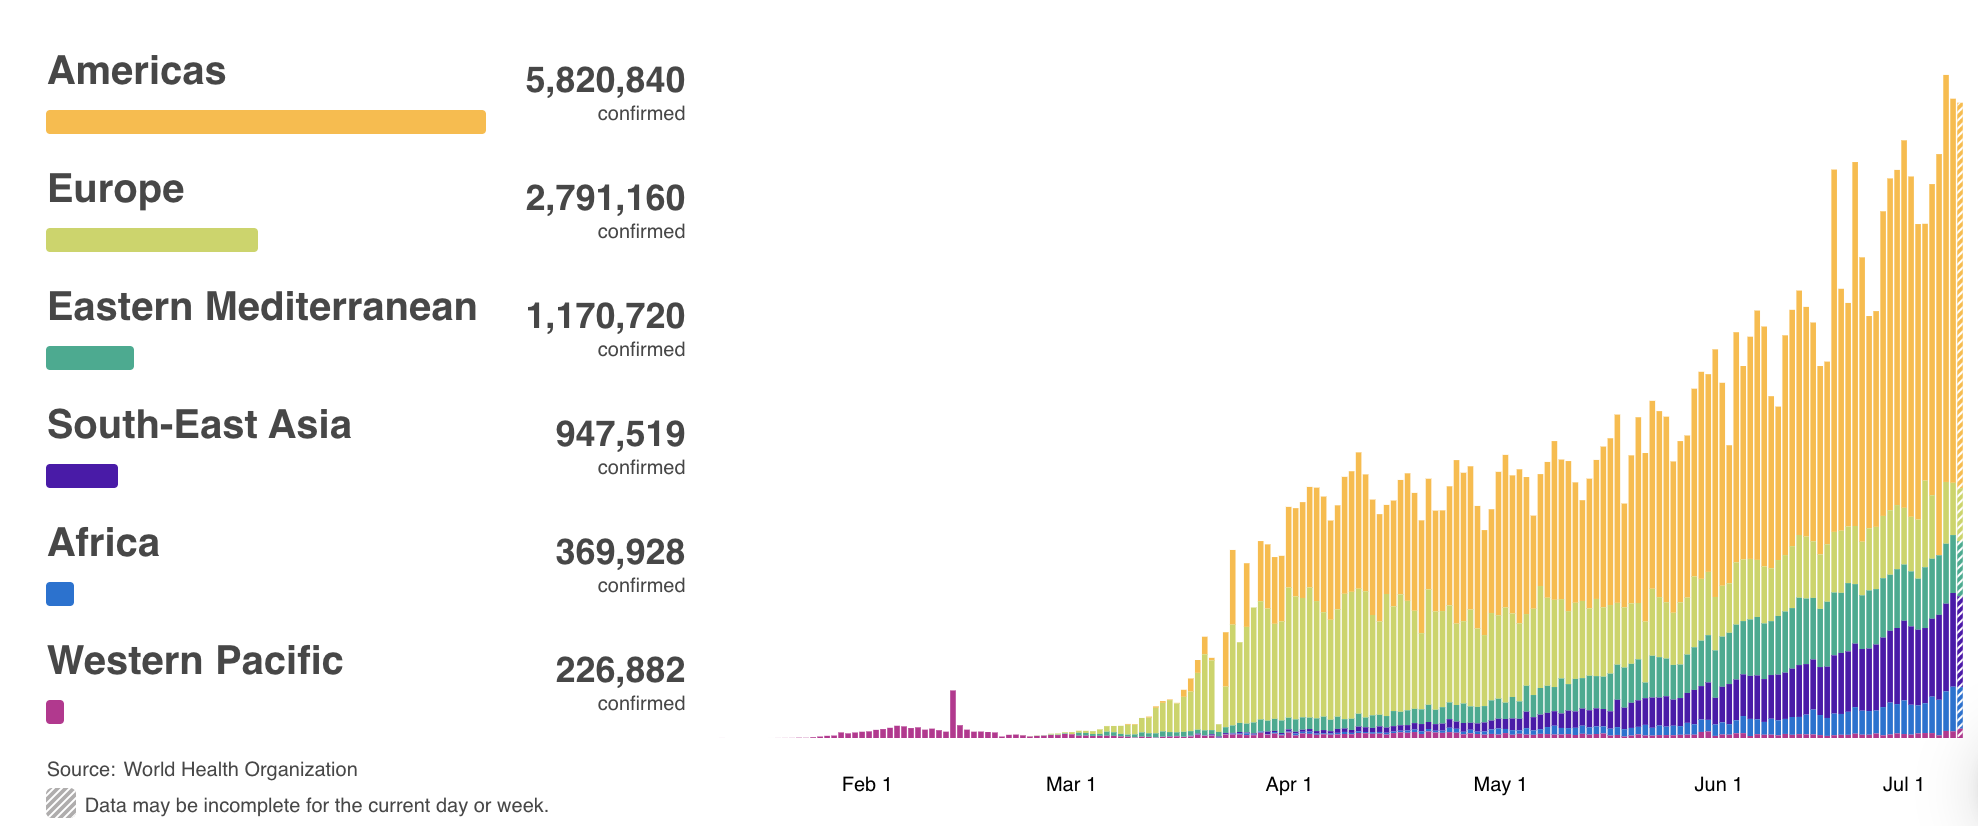
\includegraphics[]{./input/covid1.png} %插入图片,[]中设置图片大小,{}中是图片文件名
\label{} %用于文内引用的标签
\end{figure}

\begin{table}[H]
    \caption{累计确诊前十位国家}
      \vspace{-0.5\baselineskip} \begin{table}[H]
\centering\begingroup\fontsize{18}{20}\selectfont

\begin{tabular}{rlrrr}
\toprule
  & 国家(地区) & 累计确诊病例 & 总人口 & 粗发病率\\
\midrule
\rowcolor{gray!6}  1 & 美国 US & 387,547 & 331,002,651 & 117\\
2 & 西班牙 Spain & 140,618 & 46,754,778 & 301\\
\rowcolor{gray!6}  3 & 意大利 Italy & 135,586 & 60,461,826 & 224\\
4 & 法国 France & 110,049 & 65,273,511 & 169\\
\rowcolor{gray!6}  5 & 德国 Germany & 107,591 & 83,783,942 & 128\\
6 & 中国 China & 82,718 & 1,439,323,776 & 6\\
\rowcolor{gray!6}   & 湖北 Hubei & 67,803 & 59,172,000 & 115\\
7 & 伊朗 Iran & 62,589 & 83,992,949 & 75\\
\rowcolor{gray!6}  8 & 英国 United Kingdom & 55,946 & 67,886,011 & 82\\
9 & 土耳其 Turkey & 34,109 & 84,339,067 & 40\\
\rowcolor{gray!6}  10 & 瑞士 Switzerland & 22,253 & 8,654,622 & 257\\
\bottomrule
\end{tabular}
\endgroup{}
\end{table} \begin{tablenotes}
        \fontsize{15}{15}
        \selectfont
        \item 注:粗发病率定义:在一定时间内,特定范围人群中某病新发生的病例出现的频率。计算方式:(累计确诊病例/人口)×10万  %此处加入注释信息
      \end{tablenotes}
    \end{table}

\(\quad\)美国新增病例数仍居全球首位,已连续十六天日新增病例数超过两万五千人。意大利日新增病例数已经连续三日下降,西班牙和德国的日新增病例较昨日翻倍。值得注意的是,俄罗斯、巴西和比利时的病例较前日增长很快,这三个国家的累计确诊人数已突破两万例。提示欧洲、北美和南美疫情发展迅速
(表2和图2)。

\(\quad\)美国的日新增死亡病例已经接近2,500(2,494例),从4月4日至今一直为前十位国家中首位,病死率已经上升到4.5\%,疫情发展不容乐观。法国的日新增死亡病例数波动较大。今日较昨日翻倍,成为日新增死亡病例数仅次于美国的国家(1,440)例。法国病死率持续上升(12.5\%),提示该国医疗系统正面临巨大压力。意大利和西班牙的日新增死亡病例数呈波动下降趋势。英国新增死亡病例数波动上升,还有待进一步观察
(表3和图3)。

\begin{table}[H]
    \caption{日新增病例前十位国家}
      \vspace{-0.5\baselineskip}
      \centering \begin{table}[H]
\centering\begingroup\fontsize{18}{20}\selectfont

\begin{tabular}{rlr}
\toprule
  & 国家 & 当日新增病例\\
\midrule
\rowcolor{gray!6}  1 & 美国 US & 20,880\\
2 & 法国 France & 11,086\\
\rowcolor{gray!6}  3 & 德国 Germany & 4,217\\
4 & 西班牙 Spain & 3,943\\
\rowcolor{gray!6}  5 & 土耳其 Turkey & 3,892\\
6 & 英国 United Kingdom & 3,667\\
\rowcolor{gray!6}  7 & 意大利 Italy & 3,039\\
8 & 伊朗 Iran & 2,089\\
\rowcolor{gray!6}  9 & 巴西 Brazil & 1,670\\
10 & 比利時 Belgium & 1,380\\
\bottomrule
\end{tabular}
\endgroup{}
\end{table} \end{table}\begin{table}[H]
  \vspace{-7mm}
    \caption{累计死亡病例前十位国家}
      \vspace{-0.5\baselineskip}
      \centering \begin{table}[H]
\centering\begingroup\fontsize{18}{20}\selectfont

\begin{tabular}{rlrrr}
\toprule
  & 国家 & 累计死亡病例 & 较昨日 & 病死率\\
\midrule
\rowcolor{gray!6}  1 & 意大利 Italy & 17,127 & 604 & 12.6\\
2 & 西班牙 Spain & 13,912 & 571 & 9.9\\
\rowcolor{gray!6}  3 & 美国 US & 12,291 & 1,508 & 3.2\\
4 & 法国 France & 10,343 & 1,417 & 9.4\\
\rowcolor{gray!6}  5 & 英国 United Kingdom & 6,171 & 786 & 11.0\\
6 & 伊朗 Iran & 3,872 & 133 & 6.2\\
\rowcolor{gray!6}  7 & 中国 China & 3,335 & 0 & 4.0\\
8 & 荷兰 Netherlands & 2,108 & 234 & 10.7\\
\rowcolor{gray!6}  9 & 比利時 Belgium & 2,035 & 403 & 9.2\\
10 & 德国 Germany & 2,012 & 202 & 1.9\\
\bottomrule
\end{tabular}
\endgroup{}
\end{table} \end{table}

\begin{figure}[H]
\centering
\begin{minipage}[b]{0.48\linewidth}
\caption{日新增确诊病例国家趋势图\\(中国及其他前五位国家)}
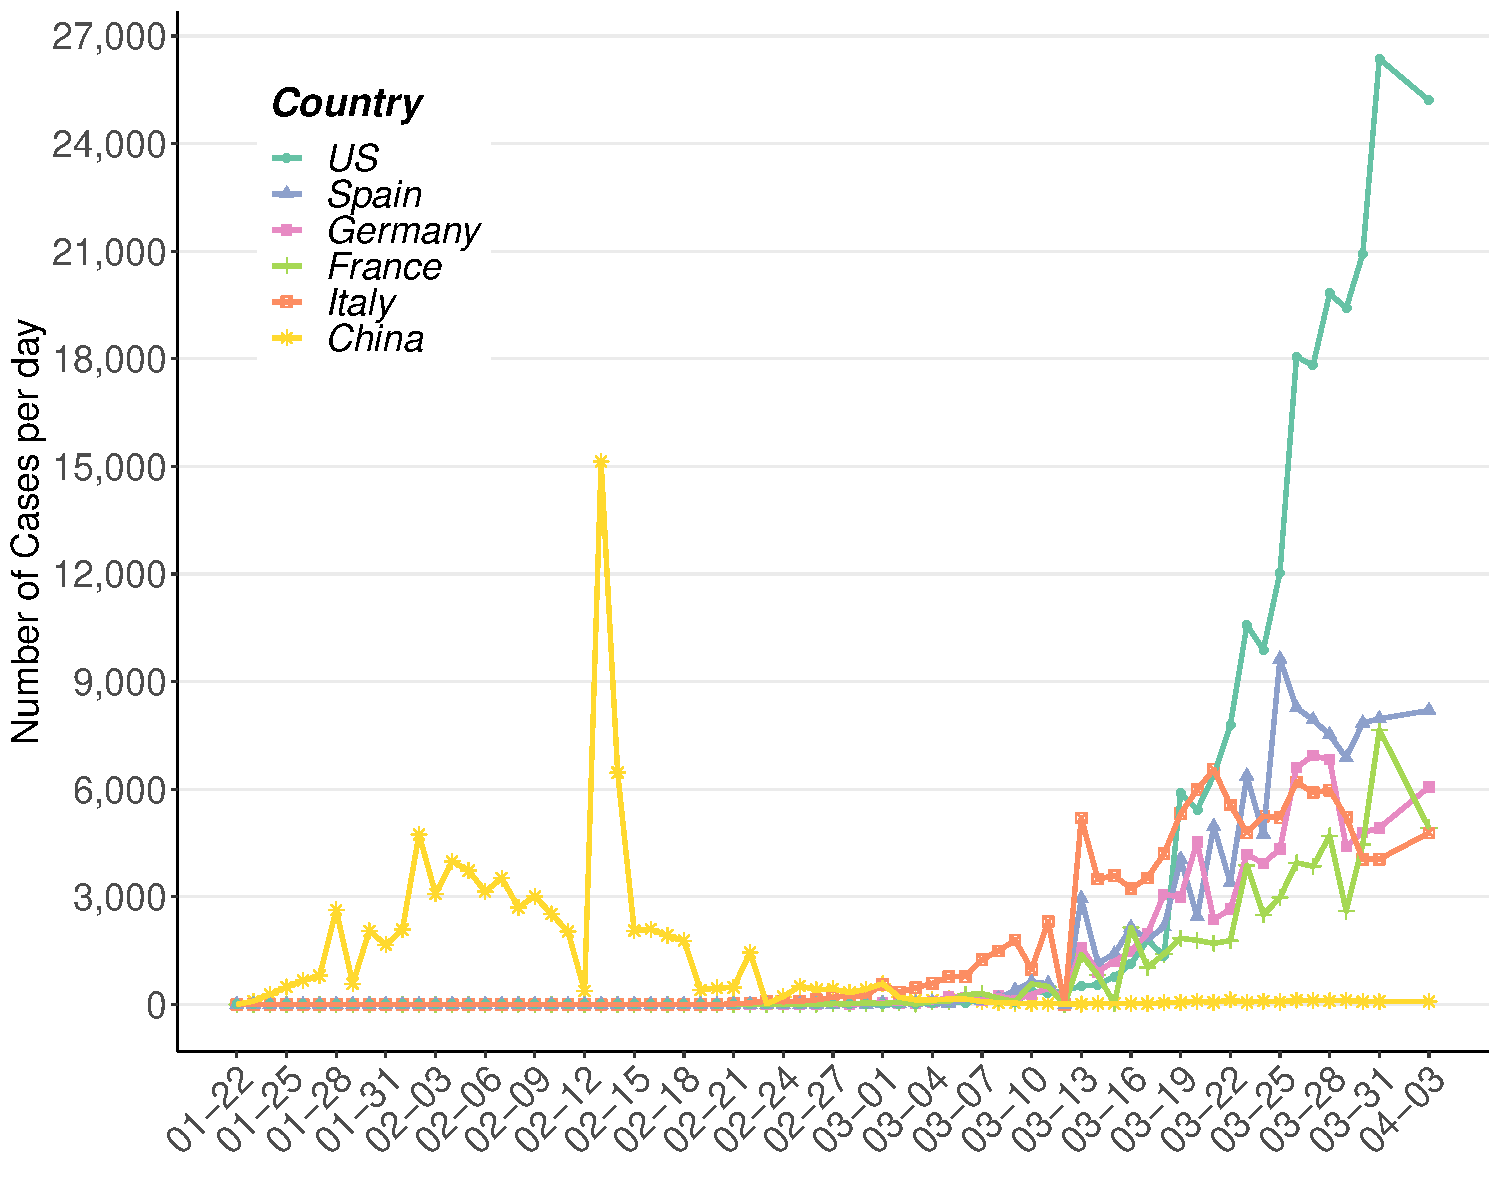
\includegraphics[]{./input/covid2.pdf}
\label{}
\end{minipage}
\quad
\begin{minipage}[b]{0.48\linewidth}
\caption{日新增死亡病例国家趋势图\\(中国及其他前五位国家) }
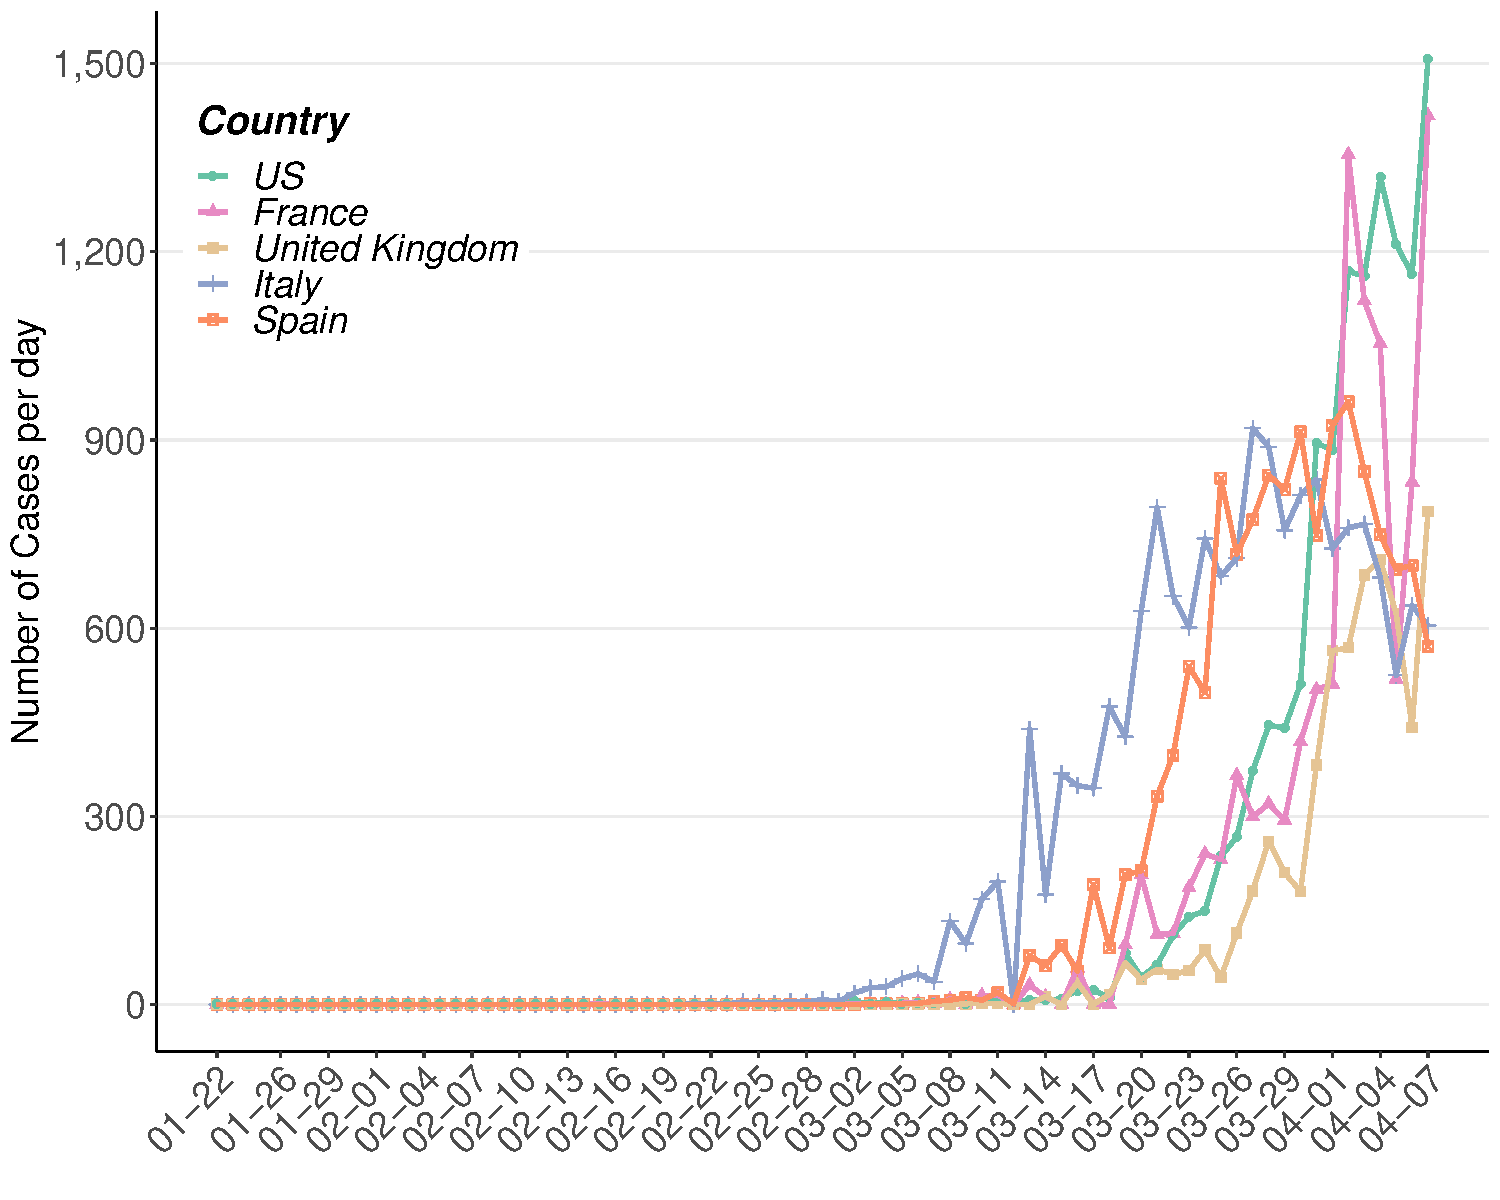
\includegraphics[]{./input/covid3.pdf}
\label{}
\end{minipage}
\end{figure}

\hypertarget{section-3}{%
\section{\texorpdfstring{\textcolor{glaucous}{\Huge 二、美国疫情}}{}}\label{section-3}}

\(\quad\)截至北京时间4月16日早7:00,
美国累计确诊病例数已达到636,350例,共28,326
死亡病例。从州疫情分布图(图4,图5)来看,美国各州疫情严重,前十州都超过一万五千人。中部地区疫情呈快速蔓延趋势。

\(\quad\)纽约州(NY)、新泽西州(NJ)和马萨诸塞州(MA)为美国疫情最严重的三个州。纽约州和新泽西州检测的阳性率仍然居高不下(40\%以上)提示两个州病人数量巨大,医疗资源持续面临巨大压力
(表4)。密歇根州(MI)的阳性率下降至31\%
(表4),提示该州的检测范围扩大,检测能力增强。

\begin{figure}[H] 
\caption{美国本土疫情分布图} %最终文档中希望显示的图片标题
\centering
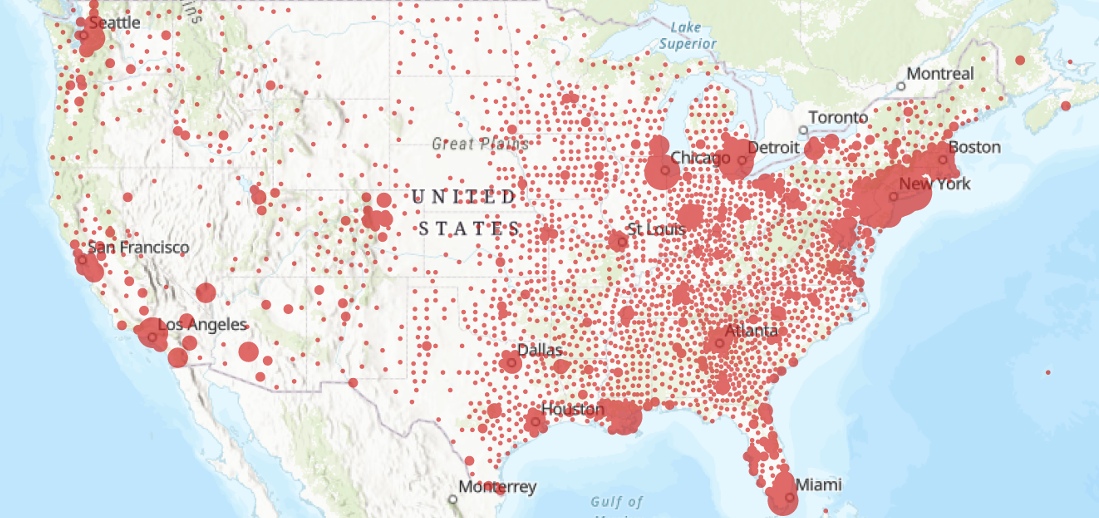
\includegraphics[]{./input/covid4.png} %插入图片,[]中设置图片大小,{}中是图片文件名
\label{} %用于文内引用的标签
\end{figure}

\begin{table}[H]
\vspace{-7mm}
    \caption{美国累计确诊前十位州}
      \vspace{-0.5\baselineskip}
      \centering \begin{table}[H]
\centering\begingroup\fontsize{12}{14}\selectfont

\begin{tabular}{rlrrrrrr}
\toprule
  & 国家/州名 & 累计确诊 & 粗发病率 & 阳性率\% & 累计检测 & 日新增检测 & 检测率\\
\midrule
\rowcolor{gray!6}   & 美国 US & 387,547 & 117 & 19 & 2,054,462 & 137,367 & 621\\
1 & 纽约州 NY & 138,863 & 714 & 41 & 340,058 & 19,247 & 1,748\\
\rowcolor{gray!6}  2 & 新泽西州 NJ & 44,416 & 500 & 47 & 94,974 & 5,942 & 1,069\\
3 & 密歇根州 MI & 17,221 & 172 & 34 & 50,332 & 3,081 & 504\\
\rowcolor{gray!6}  4 & 加利福尼亚州 CA & 16,429 & 42 & 13 & 131,229 & 13,798 & 332\\
5 & 路易斯安那州 LA & 16,284 & 350 & 22 & 74,655 & 5,489 & 1,606\\
\rowcolor{gray!6}  6 & 宾夕法尼亚州 PA & 14,852 & 116 & 16 & 91,278 & 7,424 & 713\\
7 & 佛罗里达州 FL & 14,504 & 68 & 10 & 138,162 & 14,888 & 643\\
\rowcolor{gray!6}  8 & 马萨诸塞州 MA & 13,837 & 199 & 17 & 81,344 & 4,915 & 1,171\\
9 & 伊利诺伊州 IL & 12,266 & 97 & 18 & 68,732 & 5,790 & 542\\
\rowcolor{gray!6}  10 & 乔治亚州 GA & 8,822 & 83 & 26 & 33,713 & 6,299 & 318\\
\bottomrule
\end{tabular}
\endgroup{}
\end{table} \begin{tablenotes}
    \fontsize{12}{12}
      \selectfont
    \item 注: 检测率定义:累计检测人数/10万人。计算方式:(累计检测人数/人口)*10万
    \end{tablenotes}
    \end{table}

\begin{figure}[H]
\centering
\begin{minipage}[b]{0.48\linewidth}
\caption{美国日新增确诊前五位州趋势图}
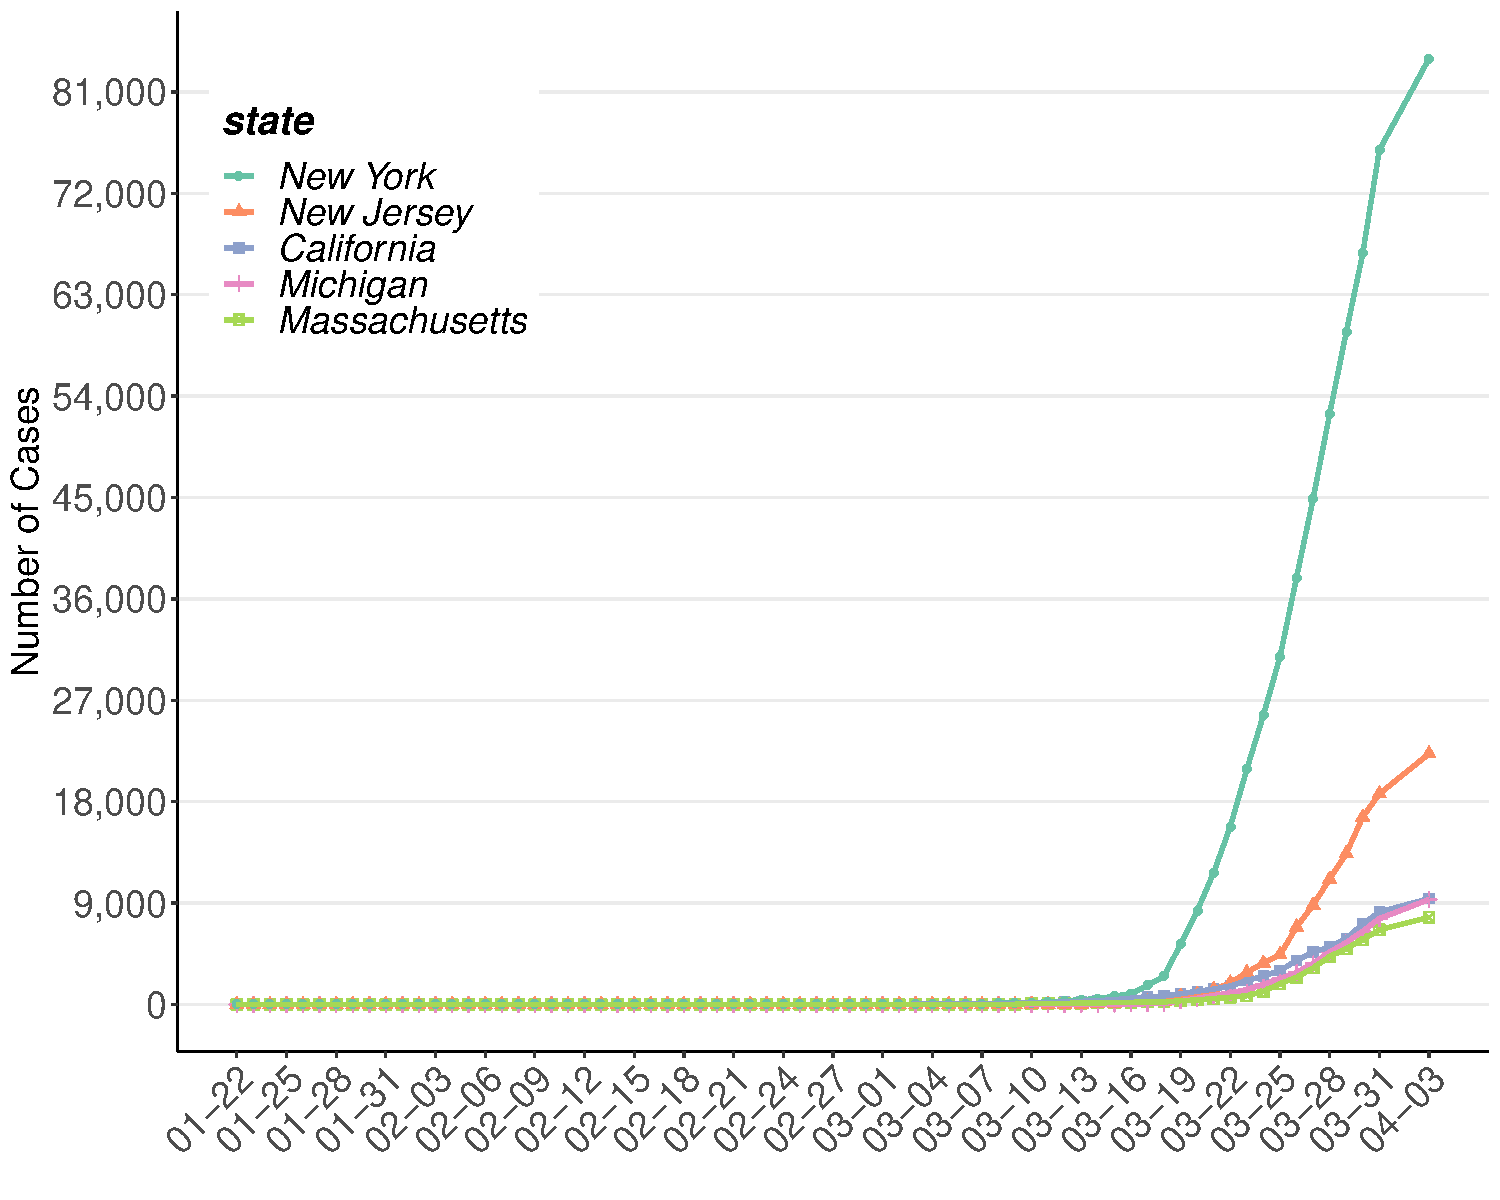
\includegraphics[]{./input/covid5.pdf}
\label{}
\end{minipage}
\quad
\begin{minipage}[b]{0.48\linewidth}
\caption{美国日新增死亡前五位州趋势图}
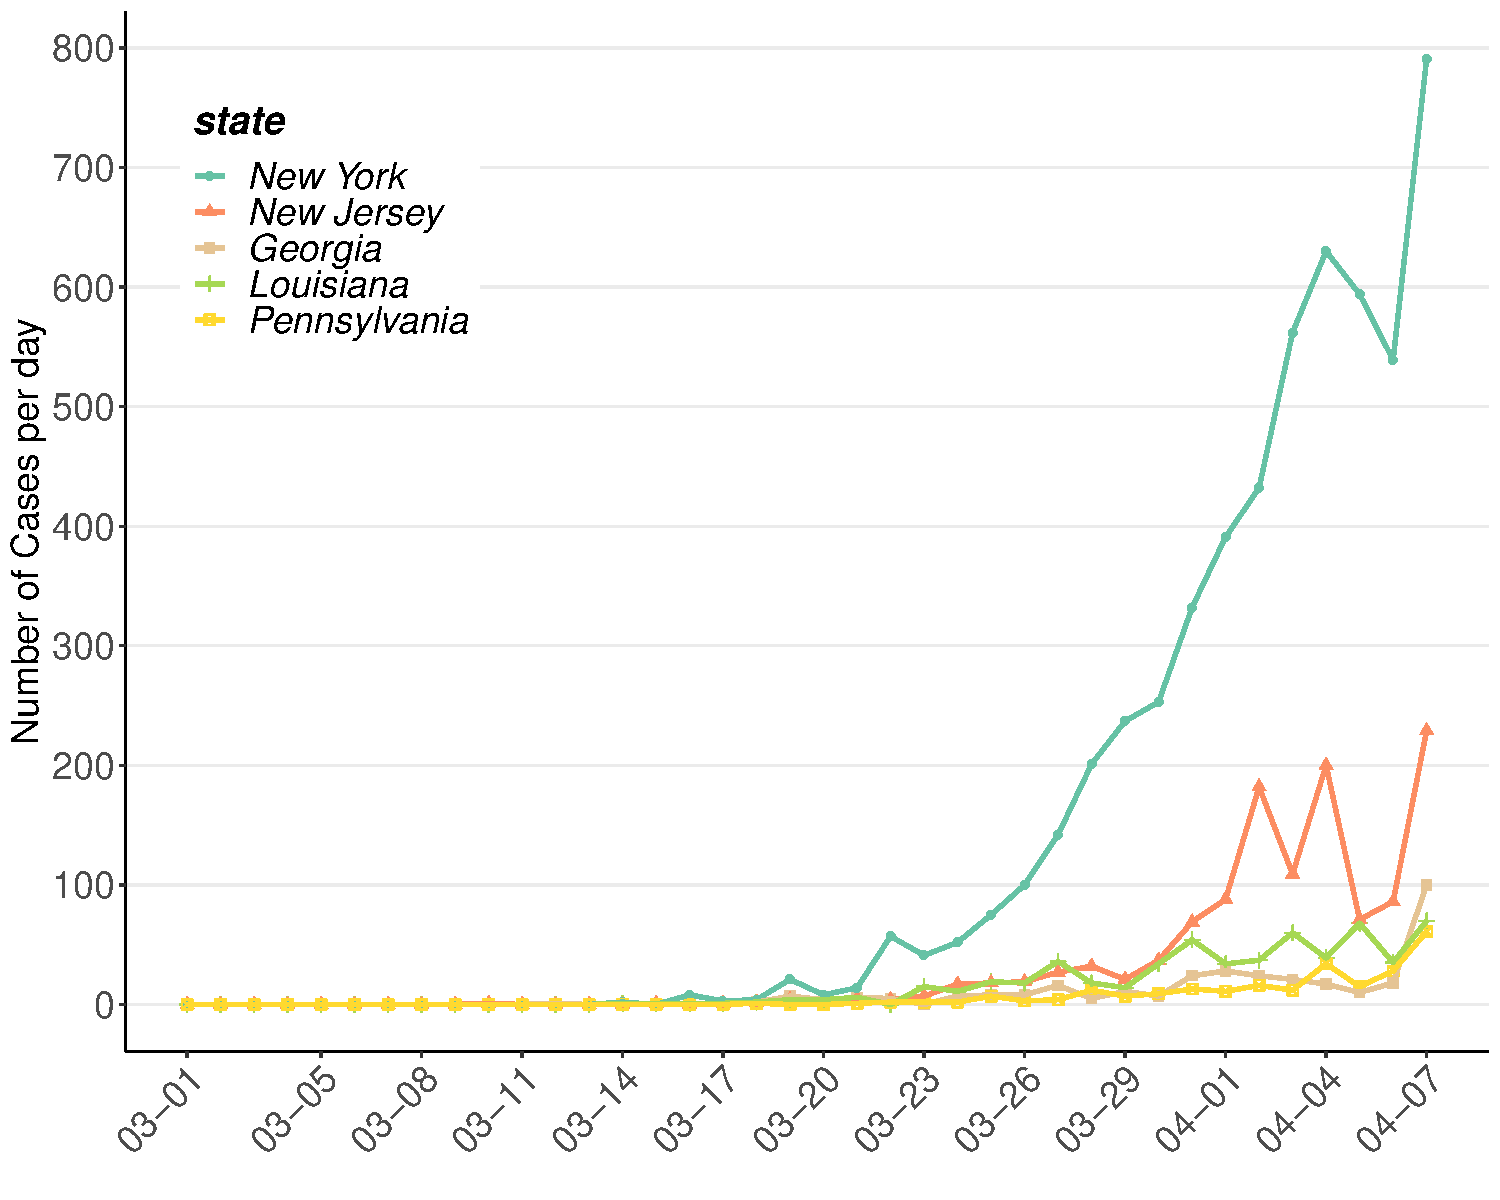
\includegraphics[]{./input/covid6.pdf}
\label{}
\end{minipage}
\end{figure}

\begin{table}[H]
    \caption{美国新增确诊前十位州}
      \vspace{-0.5\baselineskip}
      \centering \begin{table}[H]
\centering\begingroup\fontsize{18}{20}\selectfont

\begin{tabular}{rlrr}
\toprule
  & 国家/州名 & 当日新增 & 全美比率\\
\midrule
\rowcolor{gray!6}   & 美国 US & 20,880 & 100\\
1 & 纽约州 NY & 7,048 & 34\\
\rowcolor{gray!6}  2 & 新泽西州 NJ & 3,326 & 16\\
3 & 宾夕法尼亚州 PA & 1,725 & 8\\
\rowcolor{gray!6}  4 & 乔治亚州 GA & 1,508 & 7\\
5 & 路易斯安那州 LA & 1,417 & 7\\
\rowcolor{gray!6}  6 & 佛罗里达州 FL & 1,180 & 6\\
7 & 印第安纳州 IN & 554 & 3\\
\rowcolor{gray!6}  8 & 弗吉尼亚州 VA & 457 & 2\\
9 & 得克萨斯州 TX & 452 & 2\\
\rowcolor{gray!6}  10 & 加利福尼亚州 CA & 410 & 2\\
\bottomrule
\end{tabular}
\endgroup{}
\end{table} \end{table}\begin{table}[H]

    \caption{美国累计死亡前十位州}
      \vspace{-0.5\baselineskip}
      \centering \begin{table}[H]
\centering\begingroup\fontsize{18}{20}\selectfont

\begin{tabular}{rlrr}
\toprule
  & 国家/州名 & 累计死亡人数 & 病死率\\
\midrule
\rowcolor{gray!6}   & 美国 US & 12,291 & 3.2\\
1 & 纽约州 NY & 5,489 & 4.0\\
\rowcolor{gray!6}  2 & 新泽西州 NJ & 1,232 & 2.8\\
3 & 密歇根州 MI & 727 & 4.2\\
\rowcolor{gray!6}  4 & 路易斯安那州 LA & 582 & 3.6\\
5 & 加利福尼亚州 CA & 397 & 2.4\\
\rowcolor{gray!6}  6 & 华盛顿州 WA & 388 & 4.6\\
7 & 乔治亚州 GA & 329 & 3.7\\
\rowcolor{gray!6}  8 & 伊利诺伊州 IL & 308 & 2.5\\
9 & 佛罗里达州 FL & 283 & 2.0\\
\rowcolor{gray!6}  10 & 马萨诸塞州 MA & 260 & 1.9\\
\bottomrule
\end{tabular}
\endgroup{}
\end{table} \end{table}

\(\quad\)纽约州、新泽西州的新增确诊数仍高居前二,其中纽约州较前日增加大约5,000例(表5)。美国共有7个州当日新增病例超过1,000人,
除纽约州外,其余几个州的确诊病例人数近日都在波动 (图5)。

\(\quad\)美国累计死亡病例已突破二万五千例(表6)。纽约州日新增死亡人数近日以来较为稳定,新泽西州,马萨诸塞州和康涅狄格州的日新增死亡人数上升趋势明显(图6)。其他州的日新增死亡人数近日都在波动上升,提示美国疫情仍在恶化。

%
  \noindent\fcolorbox{lavenderblush}{lavenderblush}{\makebox[\dimexpr\textwidth-2\fboxsep-2\fboxrule][l]{\textbf{~\Huge 疫情观察}}}%

\hypertarget{section-4}{%
\section{\texorpdfstring{\textcolor{glaucous}{\Huge 全球卫生体系最薄弱国家之一 — 非洲:塞拉利昂}}{}}\label{section-4}}

\(\quad\)据《金融时报》报道,塞拉利昂750万人口,已有6人被确诊新冠肺炎,可塞拉利昂只有一台呼吸机。这台唯一的呼吸机在当地的一家私人医院,当地17家公立医院均无呼吸机。

\(\quad\)造成塞拉利昂防疫形势严峻的原因有很多。主要原因由如下几点:

\begin{enumerate}
\def\labelenumi{\arabic{enumi}.}
\tightlist
\item
  塞拉利昂是世界上最不发达国家之一,经济发展水平落后,医疗资源匮乏。
  1991-2001,该国经历了长达十年之久的内战。在2014年联合国开发计划署发布的人类发展指数排名中,塞拉利昂排名倒数第五。其首都弗里敦的面积只有整个国
  家的1/200,却承受着这个全国1/5人口的压力,且失业率高达70\%。2017年全国注册医生不到200名。
\item
  塞拉利昂的公共卫生体系发展不全面。塞拉利昂曾经是埃博拉病毒的重灾区,尽管在对抗埃博拉之后政府成立了公共卫生应急处理中心,但是由于国内无法量产抗疫物资,依然需要依靠外国援助来解决相关问题。
\item
  新冠疫情已经在非洲大陆快速扩散。截至4月5日,非洲已有51个国家报告出现新冠确诊病例,累计确诊人数8,736人。而两周前,非洲累计确诊人数仅为1,654
  例。在两周之内,非洲确诊人数就增长了4倍。由于防疫能力和资源有限,塞拉利昂无法同时在控制本土病例的同时兼顾严防输入型病例,使疫情防控雪上加霜\(^1\)。
\end{enumerate}

\(\quad\)我国政府长期以来支持非洲公共卫生事业的发展。早在2016年6月,中非就共同签署了《中华人民共和国商务部和非洲联盟委员会关于开展非洲疾病预防控制中心合作谅解备忘录》。2016年塞拉利昂总统欧内斯特·巴伊·科罗马访问中国时特别到访了中国疾控中心,商议中塞公共卫生技术合作相关事宜\(^2\)。

\(\quad\)目前我国国内疫情局势相对稳定,已大规模复工复产,医用防护服、医用防护口罩/面罩、测温仪、呼吸机产能已基本能满足国内需求,企业也正尽力组织扩大出口\(^3\)。在未来一段时间的抗疫物资援助和贸易上,我国相关产业可更多的将目光放在类似塞拉利昂这样的医疗资源和经济基础更加薄弱的国家。

\Large 参考文献:

\begin{enumerate}
\def\labelenumi{\arabic{enumi}.}
\item
  南财快评之全球疫情观察:从塞拉利昂看非洲防控
  ~\url{https://k.sina.com.cn/article_1651428902_626ece2602000p2bm.html?from=news\&subch=onews}
\item
  塞拉利昂总统访华,为何首站选择疾控中心?~\url{https://mp.weixin.qq.com/s/lf5e9PfSU7LF-3FiNoi72A}
\item
  工信部:中国呼吸机产能无法满足全球疫情防控需求
  ~\url{https://baijiahao.baidu.com/s?id=1663393284129099919\&wfr=spider\&for=pc}
\end{enumerate}

\centering
\fontsize{12}{12}
\selectfont
\begin{tabular}{ll}

主编:马晶  &  副主编:薛成海\,  仁晖  \\
执行责任编辑:王冠  & 责任编辑:乐昊欣\, 闫怡璇 \\
新闻组:张宁\, 张心其  & 数据分析:杜兆慧 \\
案例分析: 史珂玮  &  微信排版:韩佩瑾 \\
\multicolumn{2}{l}{可视化组:张立达\, 孙昊\, 唐星鸿\, 齐维为\, 刘逸洋\,张祺珉\,周梓淇}

\end{tabular}

\end{document}
